\documentclass{standalone}
\usepackage{tikz}
\usetikzlibrary{matrix,decorations.pathreplacing, calc, positioning,fit}
\begin{document}

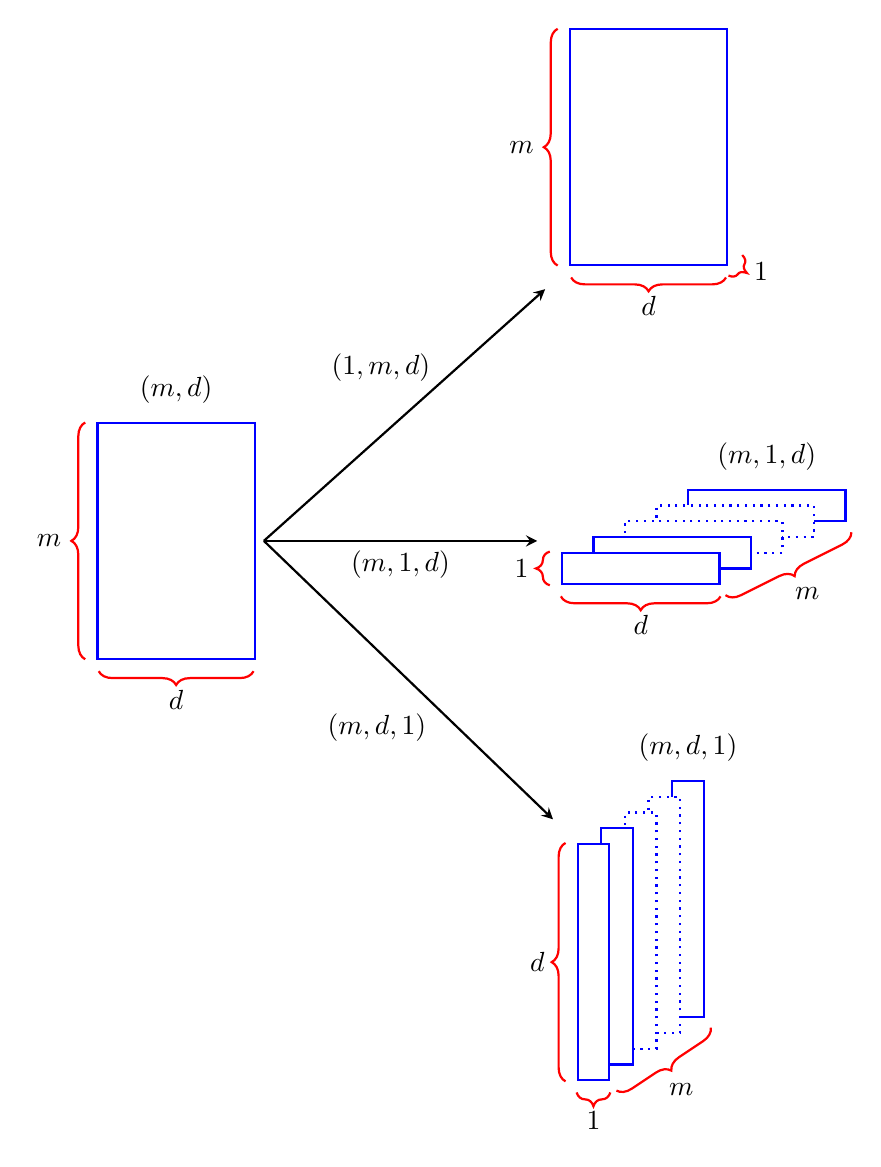
\begin{tikzpicture}[>=stealth,thick,baseline,
  mtxstyle/.style={
    draw=blue,
    minimum width=2cm,
    minimum height=3cm,
    inner sep=1pt,
    fill=white},
  vecstyle/.style={
    mtxstyle,
    minimum height=4mm},
  colstyle/.style={
    mtxstyle,
    minimum width=4mm}
    ]


\node (A) [mtxstyle] {};
\node (Alabel) [above =1mm of A.north] {$(m, d)$};
\draw [red, decorate, decoration={brace, mirror, amplitude=5pt,raise=4pt}] (A.124) -- (A.236) node [black, midway, xshift=-6mm] {$m$};
\draw [red, decorate, decoration={brace, mirror, amplitude=5pt,raise=4pt}] (A.237) -- (A.303) node [black, midway, yshift=-5mm] {$d$};

\begin{scope}[xshift=6cm, yshift=5cm]
\node (B) [mtxstyle] {};
\draw [red, decorate, decoration={brace, mirror, amplitude=5pt,raise=4pt}] (B.124) -- (B.236) node [black, midway, xshift=-6mm] {$m$};
\draw [red, decorate, decoration={brace, mirror, amplitude=5pt,raise=4pt}] (B.237) -- (B.303) node [black, midway, yshift=-5mm] {$d$};
\draw [red, decorate, decoration={brace, mirror, amplitude=5pt,raise=6pt}] (B.299) -- (B.309) node [black, midway, xshift=5mm, yshift=-2mm] {$1$};
\end{scope}

\begin{scope}[xshift=6cm]
\node (C) [xshift=15mm, yshift=4.5mm, vecstyle] {};
\node (C2) [xshift=11mm, yshift=2.5mm, vecstyle, dotted] {};
\node (C3) [xshift=7mm, yshift=0.5mm, vecstyle, dotted] {};
\node (C4) [xshift=3mm, yshift=-1.5mm, vecstyle] {};
\node (C5) [xshift=-1mm, yshift=-3.5mm, vecstyle] {};
\node (Clabel) [above =1mm of C.north] {$(m, 1, d)$};
\draw [red, decorate, decoration={brace, mirror, amplitude=5pt,raise=4pt}] (C5.180 |- C5.90) -- (C5.180 |- C5.270) node [black, midway, xshift=-5mm] {$1$};
\draw [red, decorate, decoration={brace, mirror, amplitude=5pt,raise=4pt}] (C5.180 |- C5.270) -- (C5.360 |- C5.270) node [black, midway, yshift=-5mm] {$d$};
\draw [red, decorate, decoration={brace, mirror, amplitude=5pt,raise=4pt}] (C5.360 |- C5.270) -- (C.360 |- C.270) node [black, midway, xshift=3mm, yshift=-5mm] {$m$};
\end{scope}

\begin{scope}[xshift=5cm, yshift=-5cm]
\node (D) [xshift=15mm, yshift=4.5mm, colstyle] {};
\node (D2) [xshift=12mm, yshift=2.5mm, colstyle, dotted] {};
\node (D3) [xshift=9mm, yshift=0.5mm, colstyle, dotted] {};
\node (D4) [xshift=6mm, yshift=-1.5mm, colstyle] {};
\node (D5) [xshift=3mm, yshift=-3.5mm, colstyle] {};
\node (Dlabel) [above =1mm of D.north] {$(m, d, 1)$};
\draw [red, decorate, decoration={brace, mirror, amplitude=5pt,raise=4pt}] (D5.180 |- D5.90) -- (D5.180 |- D5.270) node [black, midway, xshift=-5mm] {$d$};
\draw [red, decorate, decoration={brace, mirror, amplitude=5pt,raise=4pt}] (D5.180 |- D5.270) -- (D5.360 |- D5.270) node [black, midway, yshift=-5mm] {$1$};
\draw [red, decorate, decoration={brace, mirror, amplitude=5pt,raise=4pt}] (D5.360 |- D5.270) -- (D.360 |- D.270) node [black, midway, xshift=3mm, yshift=-5mm] {$m$};
\end{scope}

% Arrows with reshaping actions
\draw [->] ($(A.0) + (1mm, 0mm)$) -- ($(B.236)+(-3mm, -3mm)$) node [midway, above, xshift=-3mm, yshift=3mm] {$(1, m, d)$};
\draw [->] ($(A.0) + (1mm, 0mm)$) -- ($(A.east -| C5.west) + (-3mm, 0mm)$) node [midway, below] {$(m, 1, d)$};
\draw [->] ($(A.0) + (1mm, 0mm)$) --  ($(D5.west |- D5.north) + (-3mm, 3mm)$) node [midway, below, xshift=-4mm, yshift=-3mm] {$(m, d, 1)$};

\end{tikzpicture}
\end{document}